\chapter{Background}
\label{cha:bkg}




\section{How Vision is Presented in the Brain}
\label{sec:bio}

\begin{figure}
	\centering
	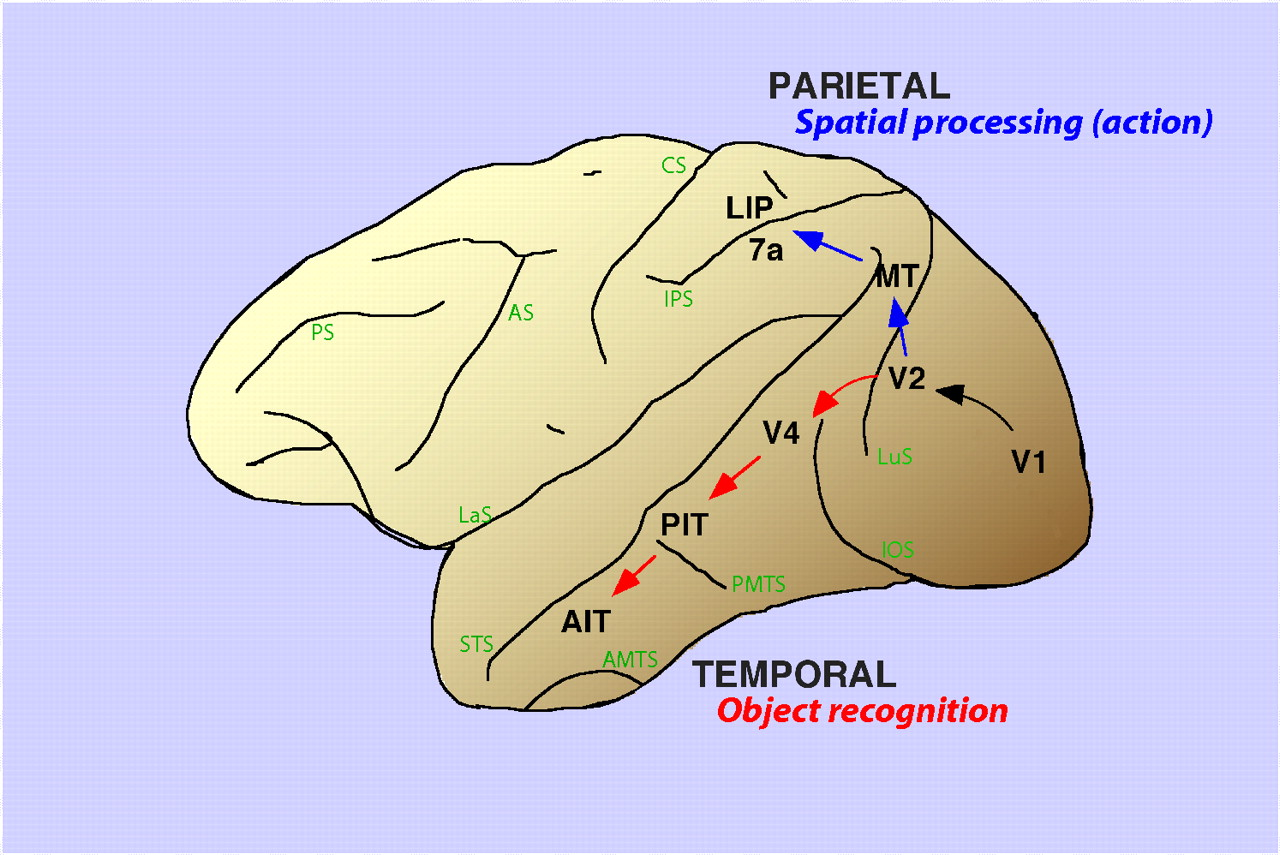
\includegraphics[width=0.8\textwidth]{pics_report/twoPaths.jpg}
	\caption{The dorsal and ventral pathway in the brain~\cite{lehky2007comparison}.
	The dorsal stream (blue) arrives to the parietal lobe, whereas the ventral pathway (red) reaches the inferotemporal (IT) cortex in the temporal lobe.}
	\label{Fig:TwoPath}
\end{figure}
The central visual system consists of several cortical areas responsible for visual processing, which are placed in a hierarchical pattern according to the anatomical experiments~\cite{felleman1991distributed}.
There are two basic streams locating in the visual area: a dorsal and a ventral pathway (Figure~\ref{Fig:TwoPath}).

They differ in behavioural patterns according to the observation from brain lesions~\cite{prado2005two}, and also in functions where the dorsal pathway targets on the `where' tasks and the ventral on the `what'.
The ventral visual stream holds the critical circuits for object recognition and stimulus identification, whereas the dorsal pathway pathway contributes to the processing of the spatial location of the stimulus~\cite{prado2005two, Ungerleider1994157}.
Another definition of the difference between these two pathways is a `perception/action' dichotomy: the ventral (`perception') stream perceives the world by means of object recognition and memory, while the dorsal (`action') stream provides real-time visual guidance for motor actions such as eye movements and grasping objects~\cite{goodale1992separate}. 

This research mainly focuses on the ventral visual pathway, since it dominates the object recognition among the cortical areas.
Thus, the dorsal pathway will beyond the scope of the this study. 


\subsection{Cortical Areas in The Ventral Visual Pathway}
The ventral visual pathway starts from the primary visual cortex V1 in the occipital cortex through areas such as V2 and V4 to the Inferotemporal (IT) cortex.
These cortex areas are divided based on the anatomical experiments and retinotopic maps.
Accordingly, the IT complex is commonly parsed into sub areas such as TEO and TE~\cite{janssen2000selectivity,von1947neocortex} or posterior IT (PIT), central IT (CIT), and anterior IT (AIT)~\cite{felleman1991distributed}.
\subsubsection{Primary Visual Cortex: V1}
As the simplest and earliest cortical area in the ventral stream, the primary visual cortex V1 is the best-studied since the well-known discovery of the orientation selectivity by Hubel and Wiesel~\cite{hubel1959receptive} in 1958.
The retinotopic map is well-defined to transform spatial information from retinal image to V1~\cite{tootell1982deoxyglucose}.
In human and animals with a fovea in the retina, the central 10 degrees of the visual field occupies roughly half of V1.
This distorted retinotopic map in V1 is a phenomenon known as cortical magnification.

\begin{figure}
	\centering
	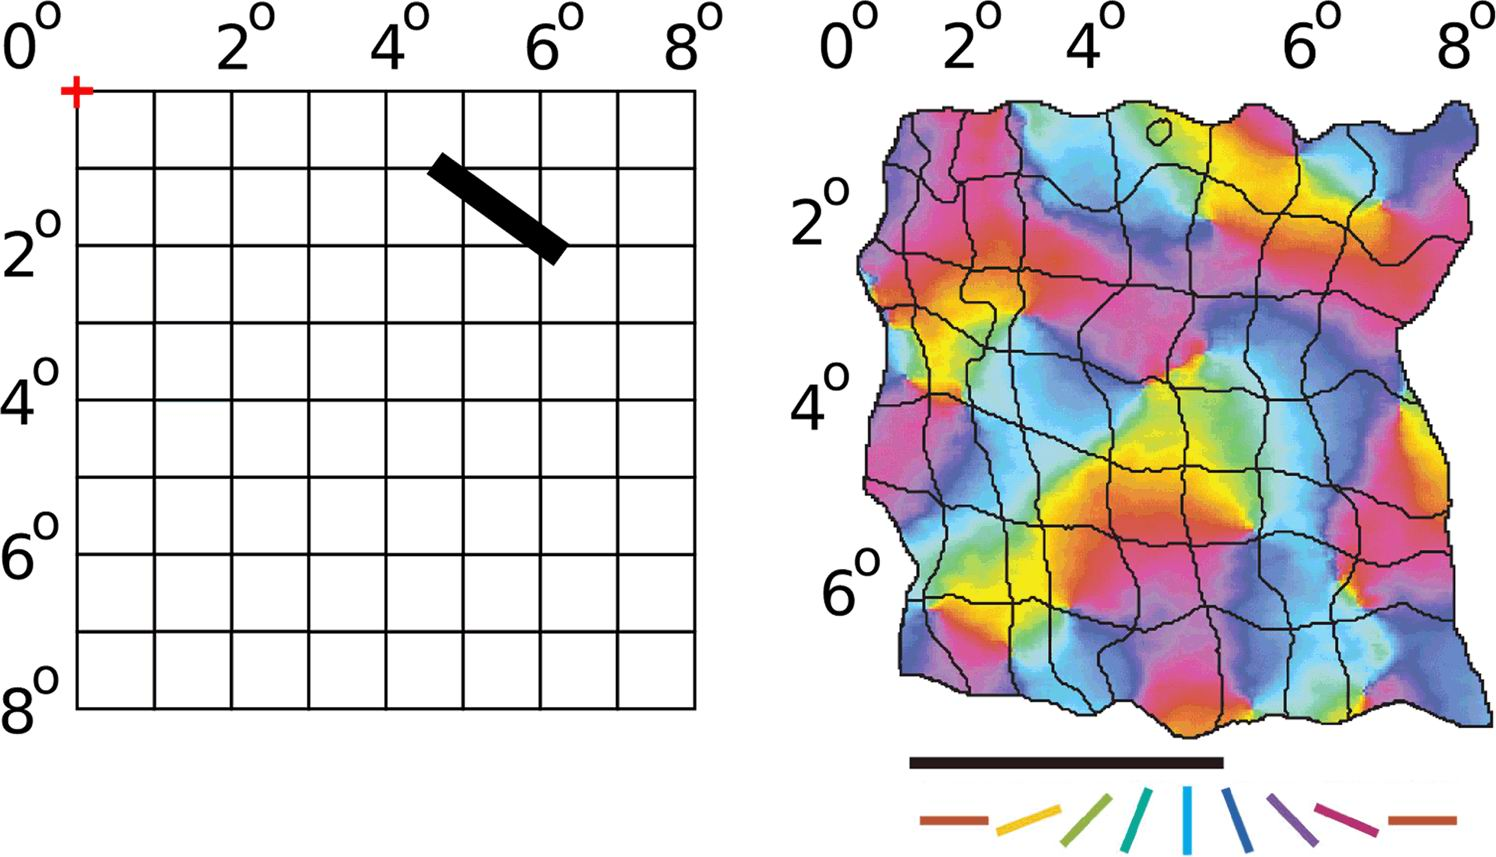
\includegraphics[width=0.8\textwidth]{pics_report/retinotopic.jpg}
	\caption{The retinotopic and orientation map on the surface of V1 of a tree shrew~\cite{bednar2009topographica}.
	The visual field (left) with a fixation point marked as a red cross on the up-left corner can be divided into a regular grid.
	Each square represents a 1$^\circ \times 1^\circ$ area of visual space.
	In cortical area V1 of mammals, neurons are arranged into a retinotopic map (right) responding to the retinal visual space.
	As an example, the retinotopic map shows the orientation preference of the V1 neurons of a tree shrew for an 8$^\circ \times 7^\circ$ area of visual space (adapted from~\cite{bosking2002spatial}; scale bar is 1 mm).}
	\label{Fig:retinotopic}
\end{figure}

In the spatial domain, V1 neurons are tuned to Gabor-like transforms applied to their small local receptive field.
The retinotopic and orientation map on the surface of V1 of a tree shrew is shown in Figure~\ref{Fig:retinotopic}.
A black bar presented in the retinal image evokes a response in the corresponding grid square of V1 (6$^\circ$, 2$^\circ$) depending on the orientation of the stimulus.
The coloured map on the right represents the preferred orientation of neurons in each location.
Thus the black bar shown at left will activate V1 neurons coloured in purple in the specific square.
In theory, these Gabor-like filters together can carry out neuronal processing of spatial frequency, orientation, motion, direction, speed, and many other spatiotemporal features.
Similar maps could be plotted for this same area showing preference for other visual features.

\subsubsection{Prestriate Cortex: V2}
Visual area V2, also called prestriate cortex~\cite{an2012distinct}, is the second major area located in the occipital lobe of the primate brain, and the first region within the visual association area~\cite{wu2011early}. 
It receives strong feed-forward connections from V1 and has many properties in common with V1. 

The responses of V2 neurons are tuned to simple shapes such as orientation and sinusoidal gratings. 
Moreover, V2 neurons are able to represent variety of higher order shapes that are based on contours (e.g., angles and curves with multiple orientations at different subregions within a single receptive field) or grating patterns~\cite{hegde2000selectivity}.
The responses of many V2 neurons are also modulated for complex properties: orientation of illusory contours~\cite{anzai2007neurons}, binocular disparity~\cite{daniel2009whither}, and whether the stimulus is part of the figure or the ground~\cite{qiu2005figure}.

%In a recent study, the Layer 6 cells of the V2 cortex were found to play a very important role in the storage of Object Recognition Memory as well as the conversion of short-term object memories into long-term memories.[23]

\subsubsection{Visual Area V4}
Area V4 is the third cortical area in the ventral stream, receiving strong feedforward input from V2 and transmitting to the PIT.
It also receives direct inputs from V1 which are mostly generated in the visual central space.
V4 is the first area in the ventral stream to show strong attentional modulation.
Most studies indicate that selective attention can change firing rates in V4 by about 20\%~\cite{filipe2013human}.
This discovery found by Moran and Desimone~\cite{moran1985selective} was the first report of attention effects anywhere in the visual cortex.

Although V4 is mainly modulated for colour recognition, it is also tuned for orientation and spatial frequency similar to V1.
Comparing to V1, V4 responds to more complex object features with intermediate complexity but is not tuned for complex objects as areas in the inferotemporal cortex are~\cite{williams2007biological}.

\subsubsection{Inferotemporal Cortex: IT}
Inferotemporal Cortex is only found in the temporal lobe in primates including humans. 
It is tuned to a range of object features complexity starting with simpler patterns in the PIT/TEO~\cite{tanaka1991coding};
And the complexity increases along the ventral stream towards AIT/TE where objects are represented and recognised~\cite{dean1976effects}.
The high-order complex features includes the combinations of colour or texture with complicated shapes~\cite{tanaka1991coding}, and body parts such as faces and hands~\cite{gross2008single}.
The distinguishing features of the IT cortex is that the neuronal responses are position and size invariant~\cite{schwartz1983shape,logothetis1995psychophysical}, and also invariant to changes in luminance, texture, and relative motion ~\cite{sary1993cue,perry2014feature}.
It is wide-accepted that the identity-preserving transformation invariance makes IT ideal for representing objects despite changes in the surrounding environment and retinal image.

In the next section, this report will explore the detailed mechanism of object representation in this cortical area.
%PFC
\subsection{Object Representation in IT}
\label{sec:orIT}
%\subsection{Untangling Object Representation}
The neuronal representation in the cortical area of IT is considered to be the spatio-temporal pattern of spikes.
The spiking activities of single neurons and populations are thought to hold the key to encode visual information.
In Section~\ref{sec:SNNintro}, the report will introduce single neuron models and spike coding mechanisms in computational spiking neural networks.

\subsubsection{Single neurons}

\begin{figure}[b!]
	\centering
	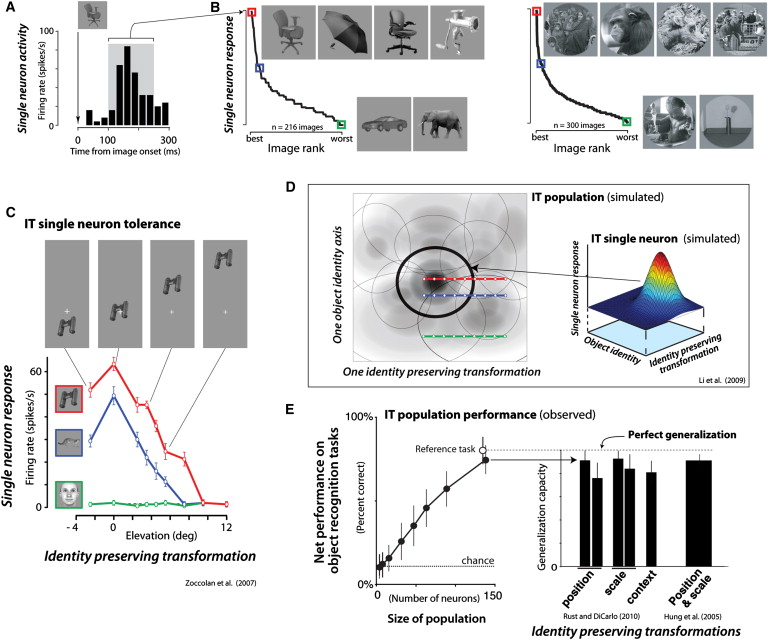
\includegraphics[width=0.9\textwidth]{pics_report/IT.jpg}
	\caption{	
		IT single-neuron properties and their relationship to population performance~\cite{dicarlo2012does}.
	}
	\label{Fig:IT}
\end{figure}
Most studies have investigated the neural activities in the IT by means of firing rate or spike count.
A typical histogram, Figure~\ref{Fig:IT}(A)~\cite{zoccolan2007trade}, shows the spike count of a single neuron in time bins of 25~ms for a duration of 300~ms in total right after the presentation of a visual image.
The highlighted time window, the so-called `decoding' window, is adjusted to the latency of the conductance along the ventral stream. 
The spike count of the `decoding' window is well modulated for object identity, position or size~\cite{desimone1984stimulus,kaneko1996sequence}, see example in Figure~\ref{Fig:IT}(B) where the left shows the spiking activities for clean figures and the right for natural scenes.
The neural responses were sorted from high to low with the corresponding figures presented, where the red point indicated the highest respond while the green the lowest and the blue the medium.
Another example in Figure~\ref{Fig:IT}(C) shows the responses of an example IT neuron obtained by varying the position (elevation) of three objects with high (red), medium (blue), and low (green) activities.
The object identity preference was maintained in the entire test range regardless of the position changes.
These tuning curves are similar to the well-understood firing rate modulation in visual area V1 on the bar orientation.

%A Contemporary View of IT Single Neurons\\
%Respond to different variations\\
%How do these IT neuronal population phenomena (above)
%depend on the responses of individual IT neurons?
Understanding IT single neuron responses has proven to be extremely challenging and even predicting the responses of an IT neuron to a new image remains impossible.
Nevertheless, IT neurons are activated by complex combinations of visual features and that they are often able to maintain their relative object preference over small to moderate changes in object position, scale, pose~\cite{logothetis1996visual}, illumination~\cite{vogels2002effects} and clutter~\cite{zoccolan2005multiple}.

%respond to more objects\\
Although IT neurons are commonly described as narrowly selective object identifier, neurophysiological studies have shown a diverse selectivity of single neurons~\cite{desimone1984stimulus}.
Most IT neurons are broadly tuned and the typical IT neuron responds to many different images and objects~\cite{zoccolan2007trade}, also see Figure~\ref{Fig:IT}(B).
As illustrated in Figure~\ref{Fig:IT}(D), a single neuron (right) is modulated to both object identities and variables of identity-preserving transformations.
To explain the plot in ~\ref{Fig:IT}(C), position is the variable here; thus the tuning curve for different identities on each position can be described as a slice in the 3-D plot which is Gaussian-like.
As a result, the rank order of the three objects remains the same due to the Gaussian-like curve stays similar.
If a population of such IT neurons tiles with the overlapping fashion, see left panel of Figure~\ref{Fig:IT}(D), a more accurate recognition result containing the transformation parameter can be carried out with population coding.

\subsubsection{Population of neurons}

Spike timing variability in the ms resolution of spikes is consistent with a Poisson-like stochastic spike generation process.
The underlying output rate of IT neurons is determined by each particular image.
Despite the timing variability, the brain can reliably recognise the presented object by integrating the neural responses across IT population~\cite{de2007properties}.
However, it still remains unclear whether the spike timing variability brings down the encoding/decoding accuracy or if it contributes to the population tuning for useful informations~\cite{ermentrout2008reliability}. 

%simple weighted summations of IT spike\\
Although the first stage of the ventral stream, V1, is reasonably well studied, the visual processing in higher stages especially in V4 and IT remains poorly understood.
Nevertheless, as stated above IT is the main part of ventral stream to recognise and categorise the objects in real-time and is tolerant to identity-preserving transformations.
Specifically, simple linear classifier built on the output rates of randomly selected population with only a few hundred neurons reveals a high-level of object recognition performance~\cite{hung2005fast};
and the simple weighted summation explains a wide range of invariant object recognition behaviour sufficiently~\cite{majaj2012unified}.

Figure~\ref{Fig:IT}(E) shows the direct tests of measuring the cross-validated population performance on categorisation tasks using linear classifiers.
The recognition performance approaches ceiling level with only a few hundred neurons (left panel), and the same population shows a good generalization across moderate changes in position, scale, and context.
%50 ms window matters\\
\subsubsection{Decoding Window Matters}
The output spiking pattern of the ventral visual stream are well described by a firing rate code where the decoding window size is 50~ms~\cite{hung2005fast}.
Thus the visual representation in IT is usually found in the first 50~ms of neuronal response, although different time epochs relative to stimulus onset may encode different types of visual information~\cite{brincat2006dynamic} (see Figure~\ref{Fig:IT}(A), an appropriate decoding window can be 100-150~ms after image onset).

%\subsection{IT}




%conclusion\\
%Such findings argue for a distributed representation of visual
%objects in IT, as suggested previously (e.g., Desimone et al.,
%1984; Kiani et al., 2007; Rolls and Tovee, 1995)—a view that
%motivates the population decoding approaches described
%above (Hung et al., 2005; Li et al., 2009; Rust and DiCarlo,
%2010). That is, single IT neurons do not appear to act as sparsely
%active, invariant detectors of specific objects, but, rather, as
%elements of a population that, as a whole, supports object recog-
%nition. This implies that individual neurons do not need to be
%invariant. Instead, the key single-unit property is called neuronal
%‘‘tolerance’’: the ability of each IT neuron to maintain its prefer-
%ences among objects, even if only over a limited transformation
%range (e.g., position changes; see Figure 4C; Li et al., 2009).
%Mathematically, tolerance amounts to separable single-unit
%response surfaces for object shape and other object variables
%such as position and size (Brincat and Connor, 2004; Ito et al.,
%1995; Li et al., 2009; Tove ́e et al., 1994; see Figure 4D). This
%contemporary view, that neuronal tolerance is the required and
%observed single-unit phenomenology, has also been shown for
%less intuitive identity-preserving transformations such as the
%addition of clutter (Li et al., 2009; Zoccolan et al., 2005).


%Summery\\
%Taken together, the neurophysiological evidence can be
%summarized as follows. First, spike counts in 50 ms IT decod-
%ing windows convey information about visual object identity.
%Second, this information is available in the IT population begin-
%ning 100 ms after image presentation (see Figure 4A). Third,
%the IT neuronal representation of a given object across changes
%in position, scale, and presence of limited clutter is untangled
%from the representations of other objects, and object identity can
%be easily decoded using simple weighted summation codes (see
%Figures 2B, 4D, and 4E). Fourth, these codes are readily
%observed in passively viewing subjects, and for objects that
%have not been explicitly trained (Hung et al., 2005). 

In sum, the output of the ventral stream is reflexively expressed in neuronal firing rates across a short interval of 50 ms and is an explicit object representation;
and the rapid production of this representation is consistent with a largely feed-forward, non-linear processing of the visual input~\cite{dicarlo2012does}, which is described in the following section.
\subsection{Hierarchical Feed-forward Organisation }
%Feed-forward, hierarchical organisation and abstraction.

\begin{figure}[h!]
	\centering
	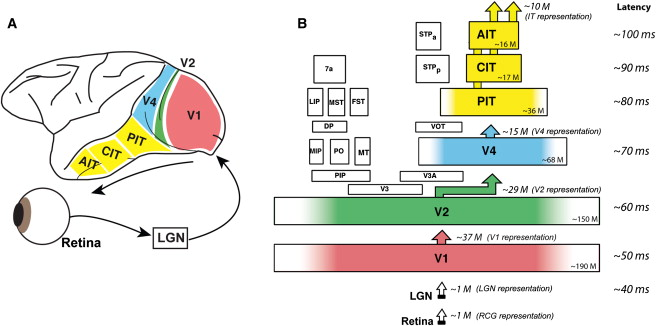
\includegraphics[width=0.9\textwidth]{pics_report/ventral.jpg}
	\caption{The ventral visual pathway and its hierarchical organization~\cite{dicarlo2012does}.
}
	\label{Fig:Ventral}
\end{figure}
Figure~\ref{Fig:Ventral}(A) illustrates the ventral stream cortical area locations in the macaque monkey brain, and the flow of visual information from the retina.
The corresponding hierarchical organisation is showed in Figure~\ref{Fig:Ventral}(B).
Each area is plotted with the size proportional to its cortical surface size.
Approximate total number of neurons of both hemispheres is shown in the corner of the cortical areas.
The approximate number of projections is written above each block.
In addition, the colour dedicates to processing the central 10$^\circ$ of the visual field.
At last, approximate median response latency is listed on the right.
%of the ventral stream with spikes travelling first from the retina to the lateral geniculate nucleus of the thalamus (LGN), and then through cortical areas introduced above: V1 , V2, V4 to IT. 
\subsubsection{Latency}
Each cortical area along the ventral stream contributes a conductance latency of about 10~ms of the visual information~\cite{nowak1997timing}.
Thus, just around 100~ms after images appeared in front of the retina, a first wave of object identity neuronal activity is present throughout much of IT (e.g., Figure~\ref{Fig:IT}(A)).

\subsubsection{Neurons and Connections}
Because retinal and LGN receptive fields are point-wise spatial sensors, the object visual information conveyed to V1 are nearly as raw as the pixel representation (1 million pixels). 
As V1 carries out its visual process, the total object representation increases approximately 30-times~\cite{stevens2001evolutionary} because of its non-linear filtering.
This dimensionality expansion results in an overcomplete population re-representation~\cite{lewicki2000learning} in which the object representation vectors have more dimensions than the LGN input.
As a result, simulations show that a V1-like representation is clearly better than RGN-like/pixel-based representation, but still far below human performance for real-world recognition problems~\cite{dicarlo2007untangling}.

The output projections of each area decreases from V2 (about 29 million) to AIT which represents the object with 10 million dimensions.
At the same time, the receptive field size of neurons increases to complete the object representation with a whole image and to perform invariant recognition.

%\begin{figure}
%	\centering
%	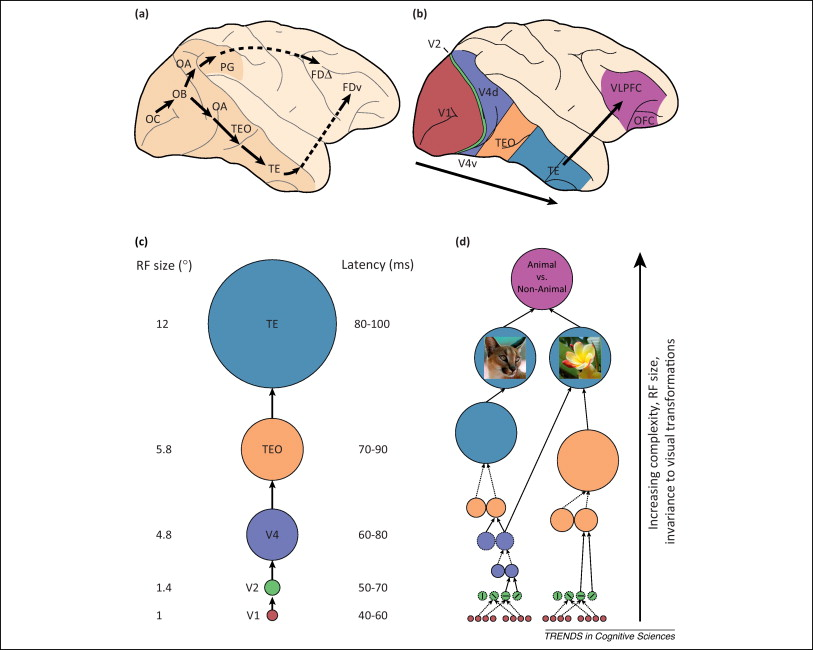
\includegraphics[width=0.9\textwidth]{pics_report/hierarchi.jpg}
%	\caption{Receptive field sizes of the sub areas along the hierarchical visual processing pathway~\cite{kravitz2013ventral}.}
%	\label{Fig:Hir1}
%\end{figure}
\subsubsection{Tuned Features and Receptive Fields }
\begin{figure}[h!]
	\centering
	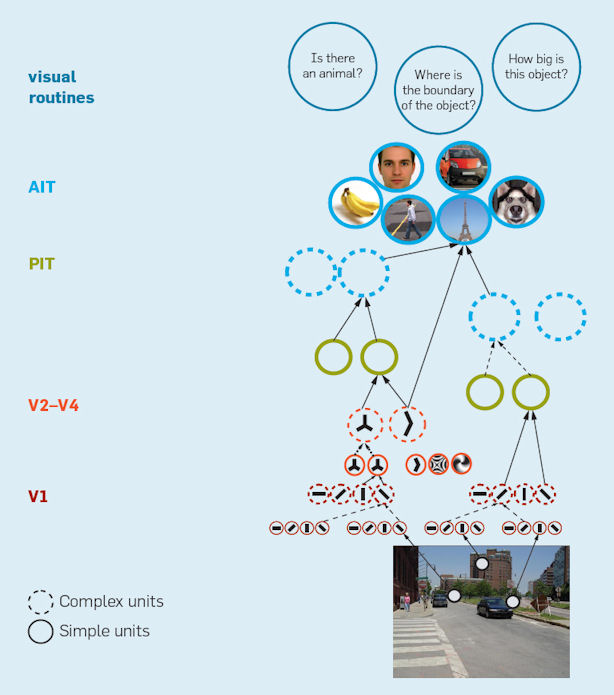
\includegraphics[width=0.9\textwidth]{pics_report/serre.jpg}
	\caption{The hierarchical ventral stream and the corresponding tuned features for each layer~\cite{serre2010neuromorphic}.}
	\label{Fig:serre}
\end{figure}
As the visual information conducts along the ventral stream, neurons become selective for stimuli that are increasingly complex from simple oriented bars and edges in early visual area V1 to moderately complex features in intermediate areas: V2, V4 and PIT to complex objects and faces in AIT, see Figure~\ref{Fig:serre}.
Along with this growing complexity of the preferred stimulus, the invariance properties of neurons also increase.
Neurons become more and more tolerant with respect to the exact position and scale of the stimulus within their receptive fields.
As a result, the receptive field size of neurons increases from
about one degree or less in V1 to several degrees in IT, see Figure~\ref{Fig:Hir1}.

\begin{figure}[h!]
	\centering
	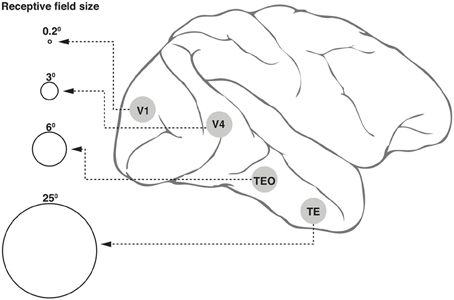
\includegraphics[width=0.6\textwidth]{pics_report/rf.jpg}
	\caption{Receptive field (RF) sizes along the ventral cortical stream in the primate. While the degree of complexity of processing may increase, the RF size at any one eccentricity also increases dramatically along the various cortical areas from V1 into the temporal pole. The circles shown in the figure are not drawn to scale, but the numbers above the circles indicate approximate relative sizes of the RF diameters.~\cite{vidyasagar2013reading}.}
	\label{Fig:Hir1}
\end{figure}

%\subsubsection{Tuned Features}
%
%V1 are orientation selective for multiple stimulus types, i.e., edges, bars, gratings (Hubel and Wiesel, 1968; Hubel et al., 1978).
%V2 cells encode border ownership (Zhou et al., 2000) which is the first stage of assigning an oriented edge to an object representation.
%Thus contour-based object representation starts in V2.
%Form processing in V4 combines multiple, spatially-adjacent, orientation responses seen in V1 and V2 to encode angles and curvatures (Pasupathy and Connor, 1999).
%These responses advance the nascent object representation from border ownership (Orban, 2008) to responses that are dependent on the placement of the curvature with respect to the center of the shape (Pasupathy and Connor, 2001).
%
%Inferior temporal (IT) cortex has a range of object property complexity starting with simpler features posteriorly (PIT or TEO: Tanaka et al., 1991; Kobatake and Tanaka, 1994) that increase in complexity as processing moves anteriorly (AIT or TE) to represent objects and perform object recognition (Cowey and Weiskrantz, 1967; Gross et al., 1971, 1972; Dean, 1976).
%This includes complex shapes, combinations of color or texture with shape (Gross et al., 1972; Desimone et al., 1984; Tanaka et al., 1991), and body parts (faces or hands: see Gross, 2008 for a review). 
%In addition, responses in IT cortex are position and size invariant (Sato et al., 1980; Schwartz et al., 1983; Rolls and Baylis, 1986; Ito et al., 1995; Logothetis and Pauls, 1995) and also invariant to changes in luminance, texture, and relative motion (Sáry et al., 1993).
%Combined, these characteristics make IT ideal for representing objects despite changes in the surrounding environment and retinal image.

%
%\begin{figure}
%	\centering
%	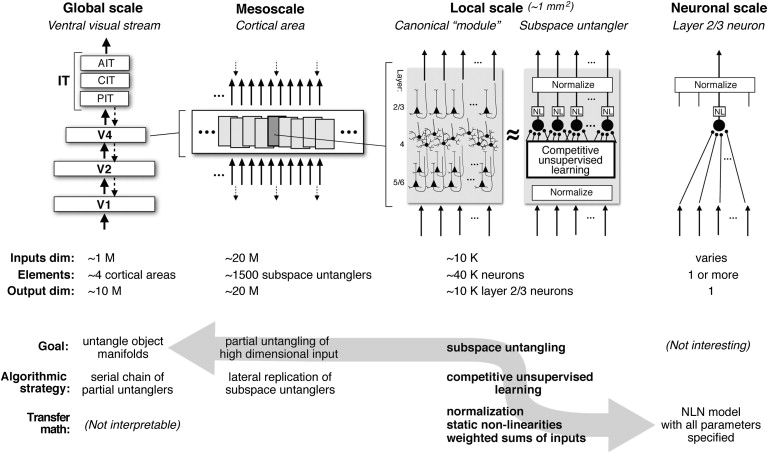
\includegraphics[width=0.9\textwidth]{pics_report/hierarchiNLN.jpg}
%	\caption{The ventral visual pathway and its hierarchical organization~\cite{dicarlo2012does}.}
%	\label{Fig:HirNLN}
%\end{figure}

\section{Computational Neuroscience: what and why spiking neurons}
\label{sec:comp}

%\section{Spatial Temporal Learning}
%\label{sec:stl}
The so-called third generation of neural networks~\cite{maass1997networks} introduces a different set of functions and parameters to model neurons;
%these both model biological neurons more precisely~\cite{hodgkin1952quantitative} and increase the computational power of networks of neurons if compared to classical sigmoidal units.
it models the biological neurons more precisely and increases the computational power of neural networks when compared to the classical sigmoid functions.
Such networks rely on the propagation of an all-or-none signal, the action potential, which asynchronously carries information to its connected units by means of its timing.
\subsection{Neuronal Model}
Spiking neuron models can be divided into two major categories \cite{gernstbook} based on their level of abstraction: The conductance models and the threshold models.
The conductance models simulate a lower level on the ion channels, while the threshold models represent a higher level of neuron abstraction where the threshold voltage is fixed and the neuron fires once the membrane potential reaches it.

In general, Conductance-Based models have been derived from the Nobel prize winners (1963) Hodgkin and Huxley, based on the experiments that they performed on the giant axon squid \cite{hhmodel}.
Spikes arriving at a LIF neuron cause a temporary flow of current into (excitatory synapse) or out of (inhibitory synapse) the neuron, modelling the behaviour of synapses in biological neurons.
The LIF neuron sums up this current over time, accumulating charge which gradually leaks away.
If the membrane potential in the neuron reaches a certain threshold, it produces a spike and its charge is reset.
LIF neurons have been extensively used in large spiking neural networks \cite{Delorme1999989} because of their ease of implementation and the low computational cost.

\subsection{Learning}
%One of the key parameters of a neural network is the amount of influence each incoming spike has on a neuron.
The influence each incoming spike has on a post-synaptic neuron is modelled by assigning a `weight' to each synapse;
tuning on the weight scales the impact of a spike
arriving via that synapse.
Many learning models simulate the changes in weights over long periods of time observed within the brain.
The exact rules by which these weights are adjusted is the subject of much active research though most promising approaches attempt to learn from the relative timing \cite{pfister2006triplets} or rate \cite{bienenstock1982theory} of spikes arriving at a neuron.
As well as adjusting weights, some learning rules can also form entirely new connections between previously unconnected
neurons \cite{bamford2010synaptic}.

\section{Neuromorphic Engineering}
\label{sec:morph}

\section{Neuromorphic Vision Recognition: State-of-the-art}
\label{sec:orec}
Researchers are using the capabilities created by rapid developments in neuromorphic engineering to address the dual aims of understanding brain functions and building brain-like machines~\cite{furber2007neural}.
Neuromorphic engineering has delivered biologically-inspired sensors such as DVS~(Dynamic Vision Sensor) silicon retinas~\cite{serrano2013128, delbruck2008frame, yang2015dynamic, posch2014retinomorphic}, which offer the prospect of low-cost visual processing thanks to their event-driven and redundancy-reducing style of information representation.
Moreover, SNN simulation tools~\cite{davison2008pynn, gewaltig2007nest, goodman2008brian} and neuromorphic hardware platforms~\cite{furber2014spinnaker,  schemmel2010wafer,benjamin2014neurogrid,merolla2014million} have been developed to allow exploration of the brain by mimicking its functions and developing large-scale practical applications~\cite{eliasmith2012large}.
In the case of visual processing, the central visual system consists of several cortical areas which, according to anatomical experiments, are placed in a hierarchical structure ~\cite{felleman1991distributed}.
Fast object recognition takes place in the feed-forward hierarchy of one of the two central visual pathways, the ventral pathway, which mainly handles the ``What'' tasks.
Biological studies have revealed that the information is unfolded along the ventral stream to the IT (Inferior Temporal) cortex~\cite{dicarlo2012does}.
Inspired by these results, SNN models have successfully been adapted to computer vision tasks.  

\cite{riesenhuber1999hierarchical} proposed a quantitative modelling framework for object recognition with position-, scale- and view-invariance.
Their cortex-like model has been analysed on several datasets~\cite{serre2007robust}.
Recently~\cite{fu2012spiking} reported that their SNN implementation was capable of recognising facial expressions with a classification accuracy (CA) of 97.35\% on the JAFFE dataset~\cite{lyons1998coding} which contains 213 images of 7 facial expressions posed by 10 individuals.
They employed simple integrate-and-fire neurons with rank order coding (ROC) where the earliest pre-synaptic spikes have the strongest impact on the post-synaptic potentials.
According to~\cite{vanrullen2002surfing}, the first wave of spikes carry explicit information through the ventral stream and in each stage meaningful information is extracted and spikes are regenerated. 
Using one spike per neuron,~\cite{delorme2001face} reported 100\% and 97.5\% accuracies on the face identification task over changing  contrast and luminance training (40 individuals $\times$ 8 images) and testing data (40 individuals $\times$ 2 images) respectively.
In terms of vision recognition on neuromorphic hardware, TrueNorth~\cite{merolla2014million} has been used to detect and recognise five classes of object in the video clips of the Neovision2 Tower dataset.
\cite{Qiao2015re} presented an analogue on-line learning neuromorphic classification system which responds selectively to images of cars and motorbikes selected from the Caltech 101 dataset.
Generic training algorithms for pattern recognition~\cite{schmuker2014neuromorphic} and regression/classification tasks~\cite{thakur2016low} have been implemented on neuromorphic platforms.

The Convolutional Neural Network (CNN), also known as the \textit{ConvNet}, developed by~\cite{lecun1998gradient}, is a widely-used model based on a cortex-like framework.
An early Convolutional Spiking Neural Network (CSNN) model identified the faces of 35 persons with a CA of 98.3\% exploiting simple integrate and fire neurons~\cite{matsugu2002convolutional}.
Another CSNN model~\cite{zhao2014feedforward} was trained and tested both with DVS raw data and Leaky Integrate-and-Fire (LIF) neurons.
It was capable of recognising three moving postures with a CA of about 99.48\% and 88.14\% on the MNIST-DVS dataset (see Chapter~\ref{sec:data}).
In a further step forward,~\cite{camunas2012event} implemented a convolution processor module in hardware which could be combined with a DVS for high-speed recognition tasks.
The inputs of the ConvNet were continuous spike events instead of static images or frame-based videos. 
The chip was capable of detecting the four suits in a 52-card deck which was browsed rapidly in only 410 ms.
Similarly, a real-time gesture recognition model~\cite{liu2014real} was implemented on a neuromorphic system with a DVS as a front-end and a SpiNNaker~\cite{furber2014spinnaker} machine as the back-end, where LIF neurons built up the ConvNet configured with biological parameters.
In this study's largest configuration, a network of 74,210 neurons and 15,216,512 synapses used 290 SpiNNaker cores in parallel and reached 93.0\% accuracy. 

Deep Neural Networks (DNNs), together with deep learning, are the most exciting research field in computer vision, but mainstream DNN research is focussed on continuous rather than spiking neural networks.
The spiking deep network has great potential to combine remarkable performance with energy-efficient training and operation.
Early research into spiking deep networks focussed on converting off-line trained deep network into SNNs~\cite{o2013real}.
The network was initially implemented on an FPGA and achieved a CA of 92.0\%~\cite{neil2014minitaur}, while a later implementation on SpiNNaker scored 95.0\%~\cite{Stromatias2015scalable}.
Recent advances have contributed to better translation by using modified units in a ConvNet~\cite{cao2015spiking} and tuning the weights and thresholds~\cite{Diehl2015fast}.
The latter paper claims a state-of-the-art performance (99.1\% on the MNIST dataset) compared to the original ConvNet.
The current trend towards training Spiking DNNs on line using biologically-plausible learning methods is also promising.
An event-driven Contrastive Divergence (CD) training algorithm for Restricted Boltzmann Machines (RBMs) was proposed for Deep Belief Networks (DBNs) using LIF neurons with Spike-Timing-Dependent Plasticity (STDP) synapses and verified on MNIST with a CA of 91.9\%~\cite{neftci2013event}.

STDP as a biological learning process has been applied to vision tasks.
\cite{bichler2012extraction} demonstrated an unsupervised STDP learning model to classify car trajectories captured with a DVS retina. 
A similar model was tested on a Poissonian spike presentation of the MNIST dataset achieving a performance of 95.0\%~\cite{diehl2015unsupervised}.
Theoretical analysis~\cite{nessler2013bayesian} showed that unsupervised STDP was able to approximate a stochastic version of Expectation Maximisation, a powerful learning algorithm in machine learning.
A computer simulation achieved a 93.3\% CA on MNIST and had the potential to be implemented using memristors~\cite{bill2014compound}. 


